\documentclass[12pt]{ctexart}

\title{控制工程基础课程设计报告}
\author{欧 宇恒}
\date{\today}
\usepackage{ctex}			%处理中文字体宏包
\usepackage{graphicx}		%处理图片宏包
\usepackage{amsmath}		%处理数学公式宏包	
\usepackage{setspace}		%处理行距宏包
\usepackage[left=1.91cm,right=1.91cm,top=2.54cm,bottom=2.54cm]{geometry}		%编辑页面格式
\usepackage{booktabs}		%处理三线表宏包
\usepackage{color}			%处理颜色宏包
\usepackage{multirow}       %处理合并单元格宏包
\usepackage{subfigure}
\usepackage{underscore}   % 处理下划线
\usepackage{listings} 
\usepackage{color}
\usepackage{indentfirst}
% -- Defining colors:
\usepackage[dvipsnames]{xcolor}
\definecolor{codegreen}{rgb}{0,0.6,0}
\definecolor{codegray}{rgb}{0.5,0.5,0.5}
\definecolor{codepurple}{rgb}{0.58,0,0.82}
\definecolor{backcolour}{rgb}{0.93,0.96,0.98}
\definecolor{codecolor}{rgb}{0.3,0.3,0.3}
% Definig a custom style:
\lstdefinestyle{mystyle}{
    backgroundcolor=\color{backcolour},   
    commentstyle=\color{codepurple},
    keywordstyle=\color{NavyBlue},
    numberstyle=\tiny\color{codegray},
    stringstyle=\color{codepurple},
    basicstyle=\ttfamily\footnotesize\bfseries\color{codecolor},
    breakatwhitespace=false,         
    breaklines=true,                 
    captionpos=t,                    
    keepspaces=true,                 
    numbers=left,                    
    numbersep=5pt,                  
    showspaces=false,                
    showstringspaces=false,
    showtabs=false,                  
    tabsize=2,
    frameround = ffff
}
% -- Setting up the custom style:
\lstset{style=mystyle, 
    language=python,}




\begin{document}	
	\ctexset{
		section={
			name={\S},
			nameformat={\zihao{3}},
			titleformat={\centering\heiti\zihao{3}},
		},
		subsection={
			name={},
			nameformat={\zihao{4}},
			titleformat={\zihao{4}},
		},
	}
\begin{titlepage}

    \begin{center}
    % Upper part of the page
    
\includegraphics[width=0.4\textwidth]{./CSU.png}\\[1cm]    
    \textsc{\LARGE Central South University}\\[1.5cm]
    \textsc{\Large Final Week Project}\\[1.5cm]
    % Title
    \textsc{\huge \bfseries 控制工程基础课程设计报告}\\[1cm]
    \textsc{\zihao{3} \bfseries 典型信号输入下一二阶系统响应仿真}\\[1.5cm]
    % Author and supervisor
    \begin{minipage}{0.4\textwidth}
    \begin{flushleft} \large
    \emph{Author:}\\
    OuYuheng
    \end{flushleft}
    \end{minipage}
    \begin{minipage}{0.4\textwidth}
    \begin{flushright} \large
    \emph{Supervisor:} \\
    Dr.Xiao \textsc{Yougang}
    \end{flushright}
    \end{minipage}
    \vfill
    % Bottom of the page
    {\large \today}
    \end{center}
    \end{titlepage}
\newpage
\tableofcontents
\newpage

\section{课程设计要求}

APPdesign 设计人机界面,能直观显示脉冲、阶跃、斜坡及不同频率正弦信号作用下,一二阶系统的输出响应,得出一二阶系统参数变化对系统输出的影响规律,并显示系统的快速性及准确性指标。

\section{系统设计思路}

通过分析项目需求,本项目通过 Python 的 CustomTkinter 库建立了前端 GUI 架构与所需控件,设计后端算法调用前端框架中的变量值,绘制输出响应的仿真曲线,计算系统快速性与准确性指标。相较于 MATLAB 提供 Appdesign 框架,Python 的 CustomTkinter 库控件更为美观、易用,如 Slider 控件在设计上响应更为迅速,并且由 Python 构建出的 GUI 框架能以较小的体积打包成 .exe 文件,便于用户使用访问,综合各方面考虑,本次课程设计采用了 Python 作为编程语言。

\subsection{前端 GUI 框架设计}

本项目在设计时,根据项目需求与功能需要,设计前端 GUI 框架如图\ref{figure1}所示,方便后续程序开发。前端 GUI 框架设计共分为组件设计、面板设计和功能设计三个部分,各部分思路图见图\ref{figure2}所示。

\begin{figure}[htbp]
    \centering
    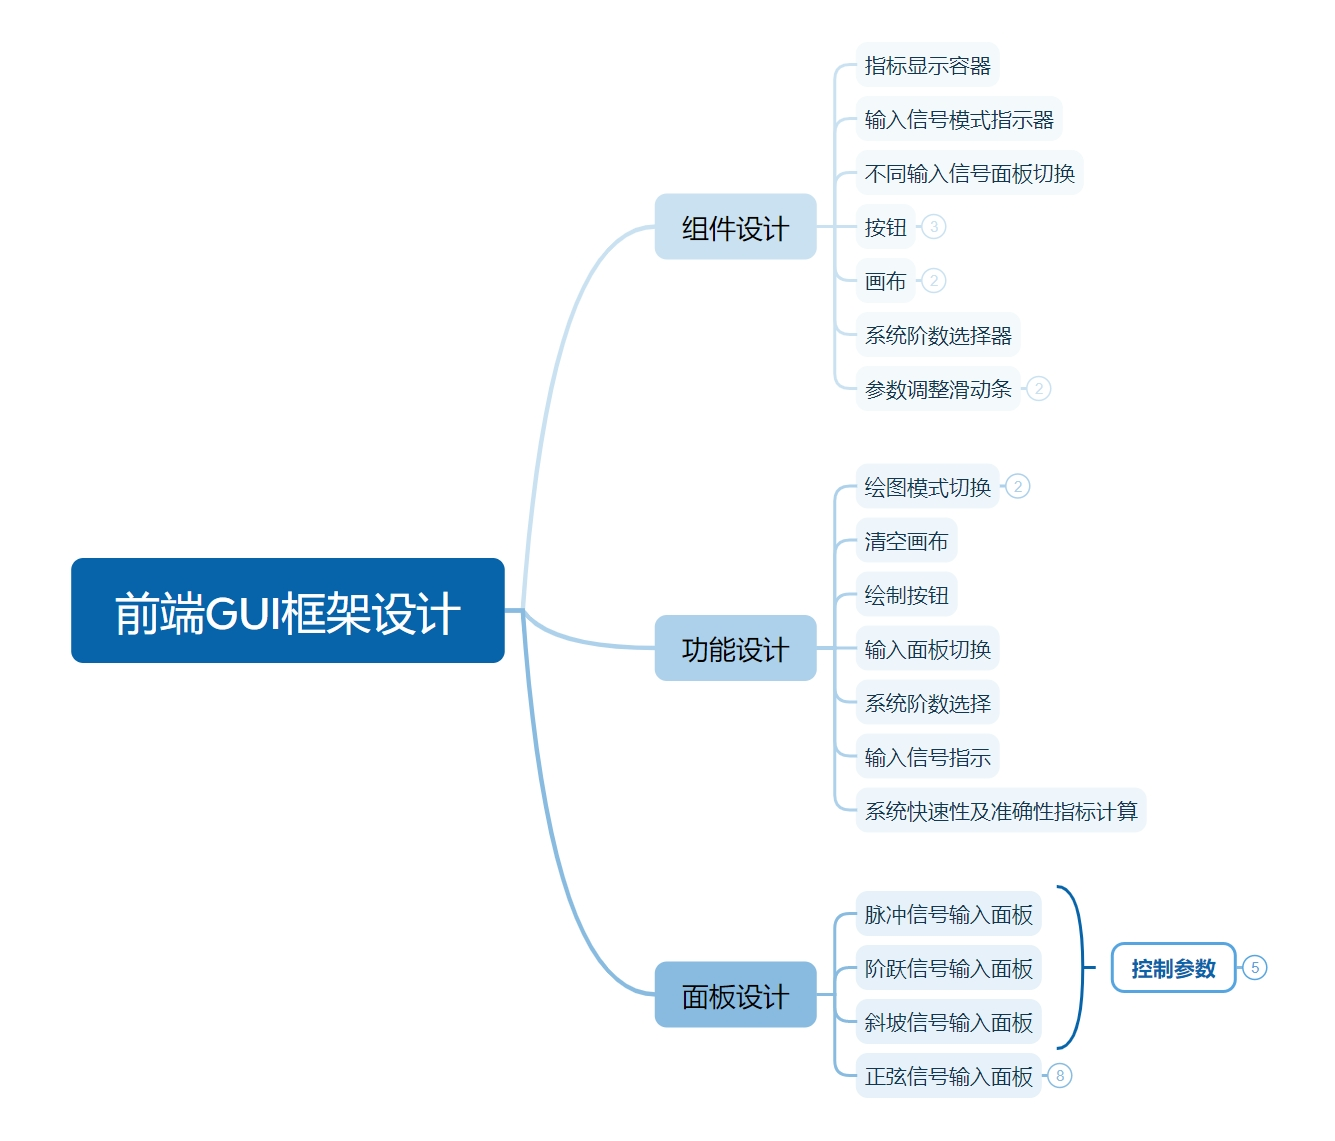
\includegraphics[width=0.7\textwidth]{img/major_framework.png}
    \caption{前端 GUI 框架设计总思路}\label{figure1}
\end{figure}
\begin{figure}[htbp]
    \centering
    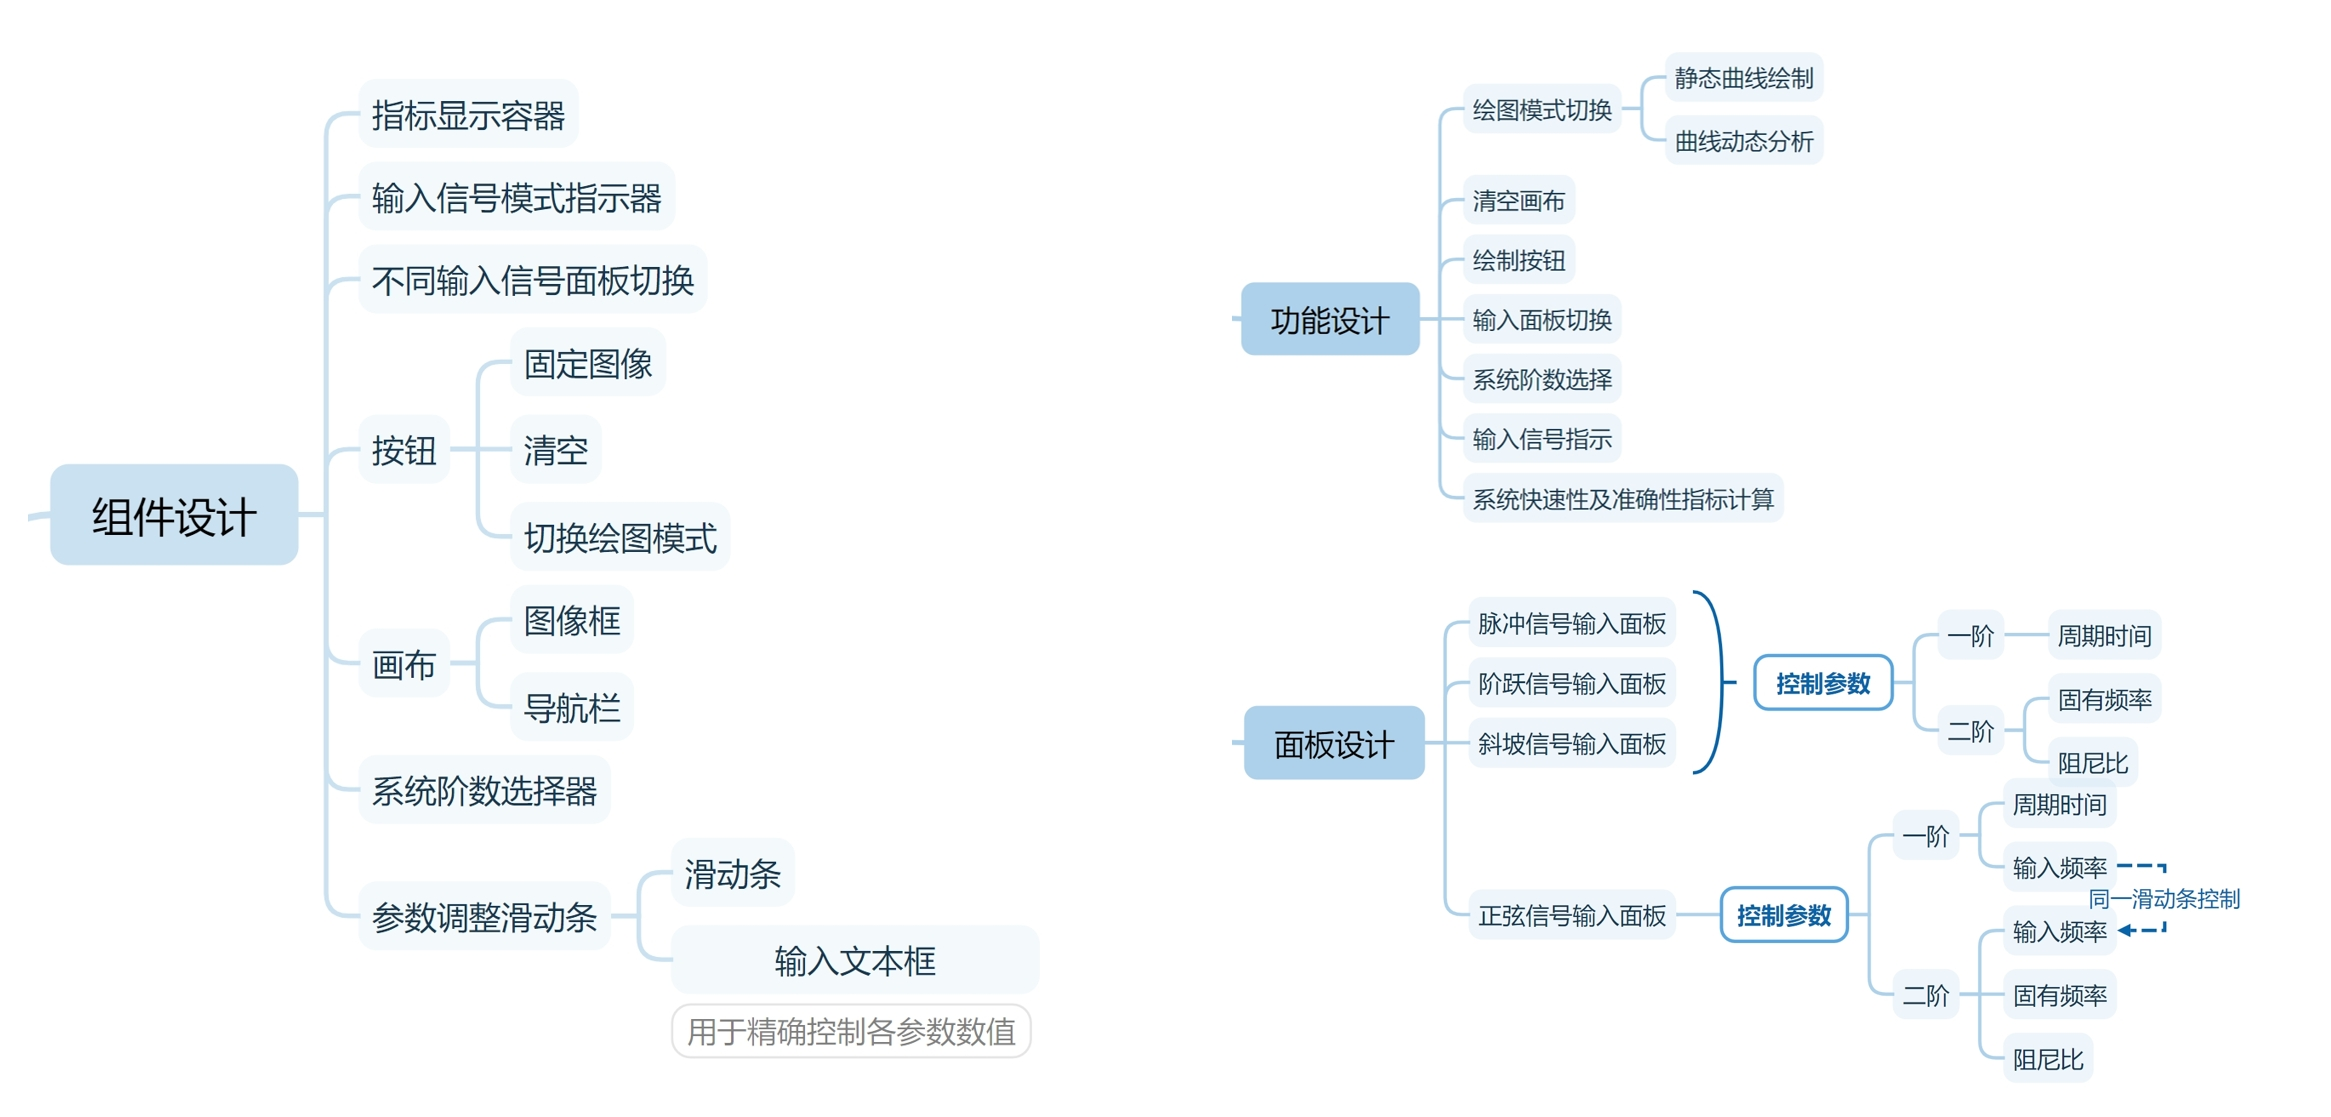
\includegraphics[width=\textwidth]{img/word_align.png}
    \caption{组件设计、功能设计、面板设计思路图}\label{figure2}
\end{figure}

在组件设计中,本项目基于 CustomTkinter 原生库设计了\texttt{Indicator, metric, MyButton, MyCanvas, MyOrder, MySliderBlock, Sin_MyOrder, tab_frame, Sin_tab_frame} 九大控件,方便后续在各个输入面板中设置需要的组件。

在面板设计中,本项目将四种输入信号设置成四个独立的面板,分为单位脉冲输入信号,单位阶跃输入信号,单位斜坡输入信号,单位正弦波输入信号,其中,各个面板下均有面板输入信号指示器,系统阶数选择器,系统参数滑动调节器与对应的图像画布和图像控制器。

在功能设计中,本项目设计了两种绘图模式,在\textbf{静态曲线绘制}中,本项目通过\texttt{caculate}按钮为用户提供曲线绘制功能,不同参数系统的响应曲线会在右侧画布中显示,配合图例标注,用户可清晰地比较多条曲线间的趋势、峰值等差异;在\textbf{曲线动态分析}模式下,本项目支持用户通过拖动滑动调节器,实时观察系统响应曲线的变化,利于动态分析。本项目通过静态与动态的功能设计,拓展了该典型信号输入下的一二阶系统响应仿真项目的应用场景。

\subsection{后端算法设计}

图像绘制中,本项目通过调用前端接口访问用户自主调节的数据,将各个参数输入系统模型,再将输入信号与系统传递函数进行拉普拉斯变换,求解在 s 域下的输出响应函数,将该函数进行反拉普拉斯变换后,通过 matplotlib 库相关函数进行输出,即可得到系统响应曲线图像,最终通过控制工程基础所学知识,计算出系统准确性与快速性响应指标,后端算法流程见图\ref{figure3}所示。

\begin{figure}
    \centering
    
\includegraphics[width=\textwidth]{img/back_design.png}
    \caption{后端算法流程}\label{figure3}
\end{figure}

\section{系统功能简介}

\subsection{Run}

\begin{lstlisting}
    git clone https://github.com/dream-oyh/Control_Engneering_Twice_Work_Python.git
    cd Control_Engneering_Twice_Work_Python
    poetry install
    poetry run python main.py 
\end{lstlisting}

请确保 PC 已经安装了 poetry 和 tkinter,若未安装 poetry 包管理器,对 archlinux 用户,请运行:

\begin{lstlisting}
    sudo pacman -S python-poetry tk 
\end{lstlisting}

对 windows 用户:

\begin{lstlisting}
    pip install poetry -i https://pypi.tuna.tsinghua.edu.cn/simple
\end{lstlisting}

若 PC 上无法运行 pip 或 python,直接运行\texttt{“dist/main/main.exe”}即可,该项目已通过 Pyinstaller 打包成 exe 可执行程序。

\subsection{Usage}

\subsubsection{界面介绍}

在本项目顶部,用户可依次选择“Pulse Input(脉冲输入)”“Step Input(阶跃输入)”“Slope Input(斜坡输入)”“Sin Input(正弦输入)”,确定输入信号类型,如图\ref{figure4}所示,同时页面左上角的图像实时反映了选择的输入模式,并显示了输入函数的图像。本系统所示输入均为单位输入,并没有考虑对系统输入的振幅进行调整。

\begin{figure}
    \centering
    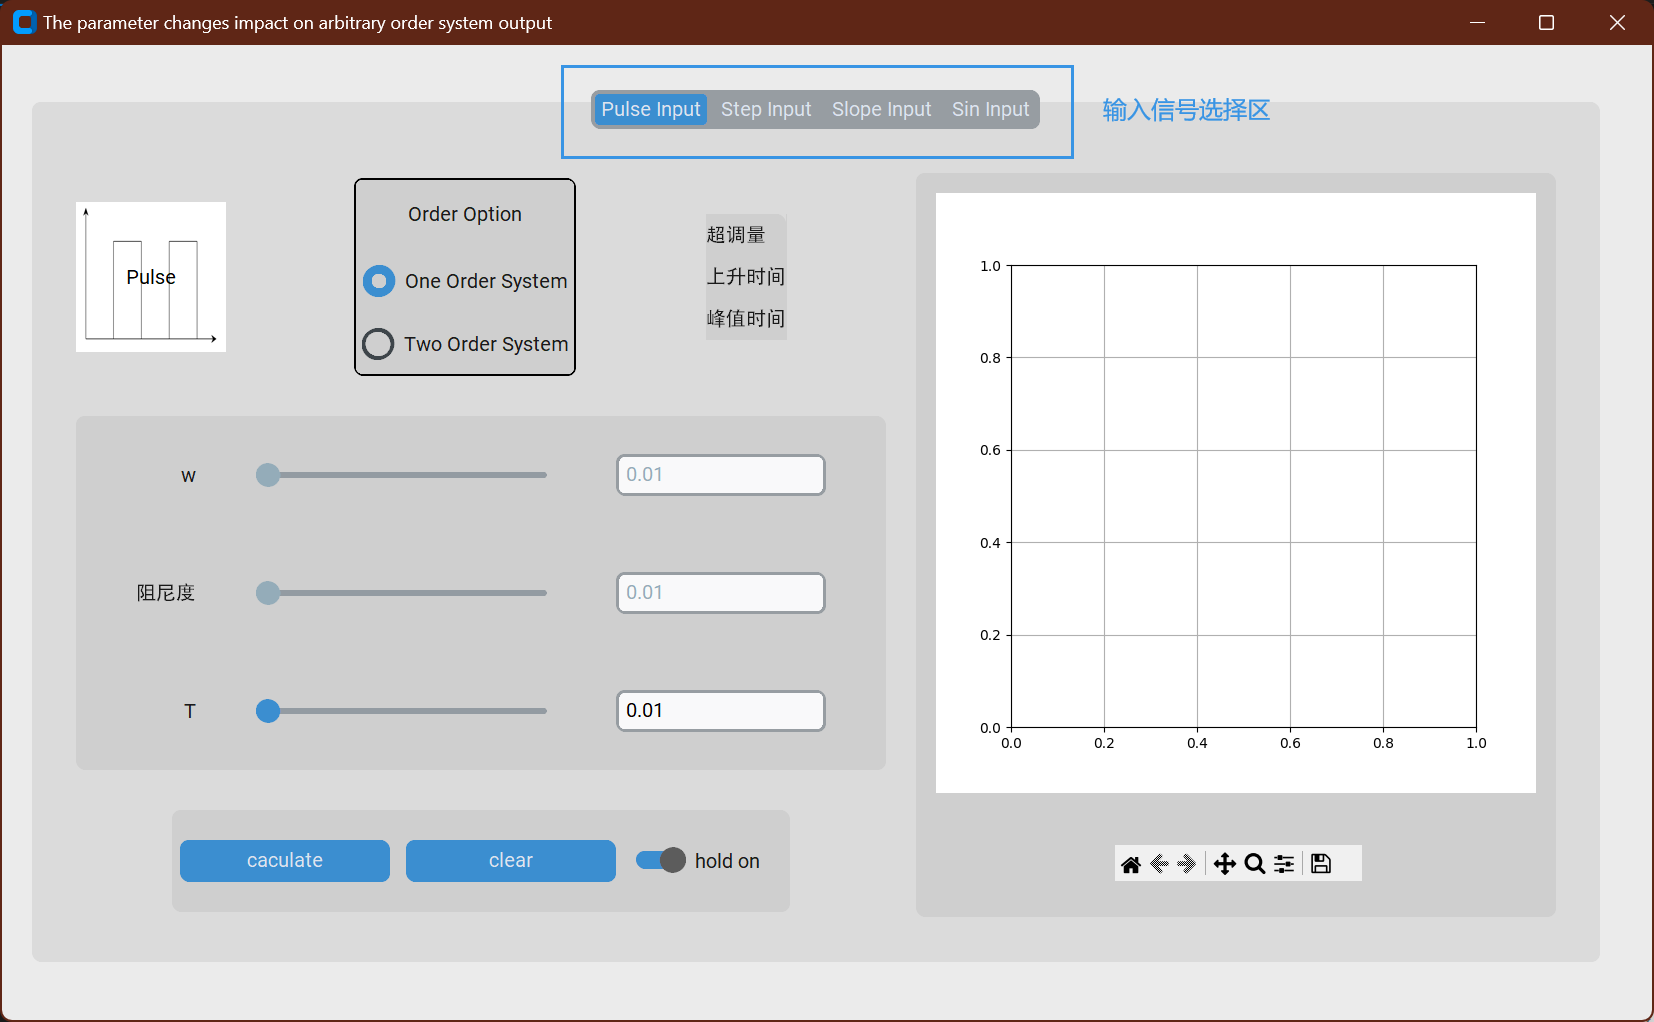
\includegraphics[width=0.7\textwidth]{img/input_signal_choose.png}
    \caption{输入信号选择}\label{figure4}
\end{figure}


Order Option 系统阶数选择器中可以选择系统的阶数,本系统提供了一阶系统(“One Order System")与二阶系统(“Two Order System”)两种系统阶数,在选择阶数后,下方相应的滑动条也会变灰,显示为不可用状态,高亮的滑动条表示了在该阶数下可以调节的参数值,如图\ref{figure5}所示。

\begin{figure}[htbp]
    \centering
    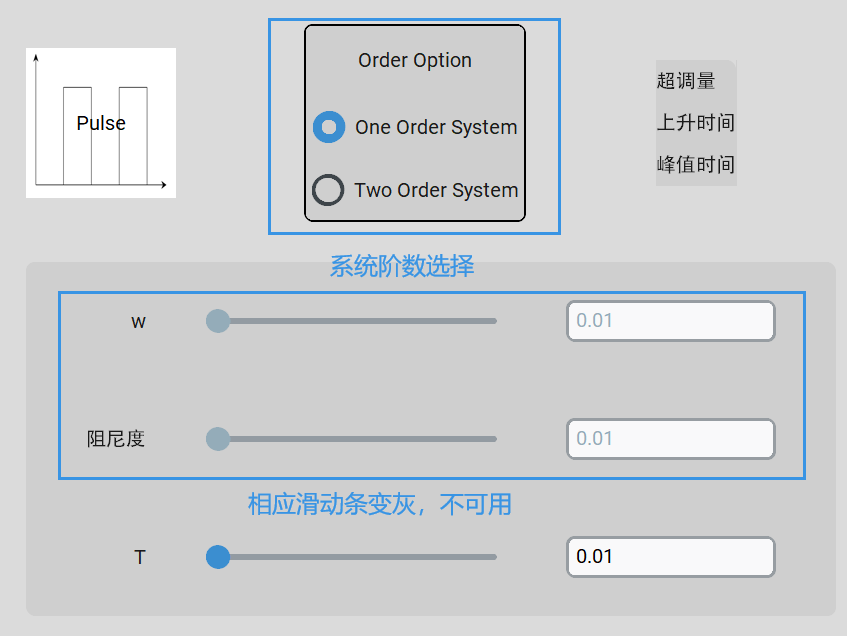
\includegraphics[width=0.4\textwidth]{img/order_option.png}
    \caption{系统阶数选择}\label{figure5}
\end{figure}

系统阶数选择器右侧可实时显示反映该系统准确性与快速性的状态量,本系统提供了“超调量”“上升时间”与“峰值时间”的计算。

下方滑动条与三个按钮可对右侧曲线图像进行操作,操作方法见“系统使用”部分,此处不再赘述。

右侧曲线图像可以比较不同参数的输出图像或实时显示响应曲线,取决于“hold on”按钮的状态,下方的导航栏可以对图像进行一定的移动和变换,如图\ref{figure6}。

\begin{figure}[htbp]
    \centering
    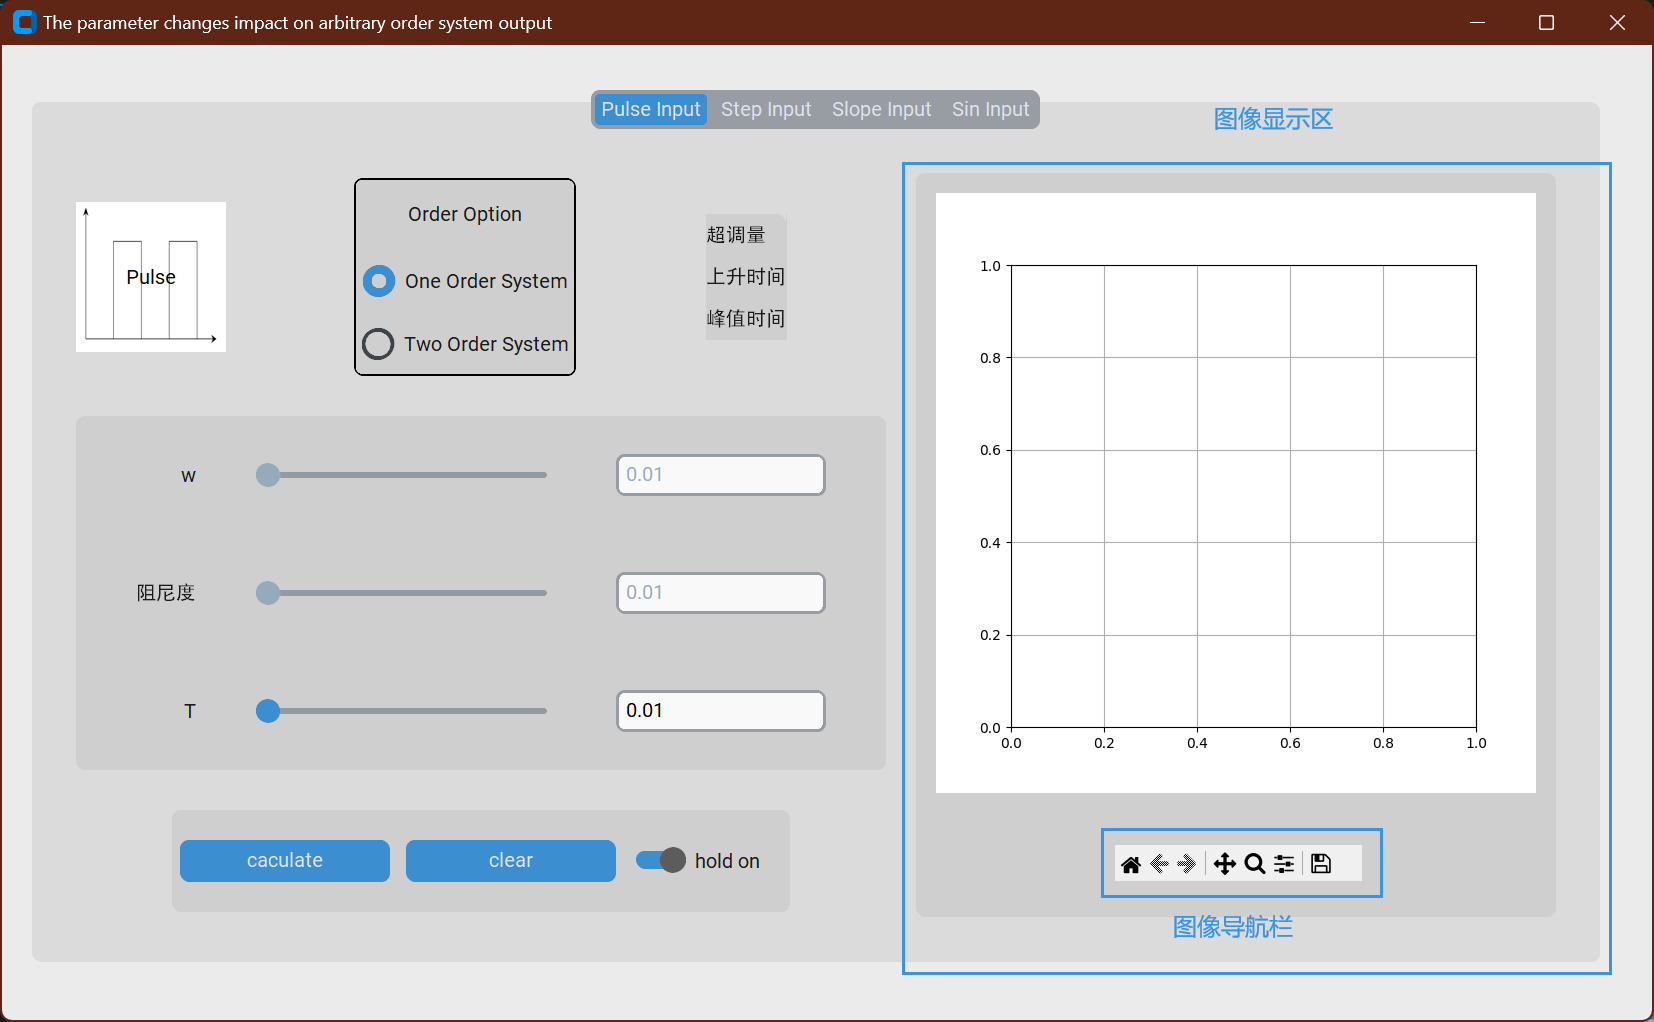
\includegraphics[width=0.7\textwidth]{img/plot_display.png}
    \caption{图像显示区}\label{figure6}
\end{figure}

\subsubsection{系统使用}

本系统设计了两个功能模式:

1. 静态曲线绘制模式:固定不同参数的响应曲线在右侧图像中,以直观地比较不同参数对响应曲线的影响;

2. 曲线动态分析模式:跟随滑动条变化实时显示响应曲线的动态变化过程,能够更好地展示在参数变化过程中曲线的动态变化。界面通过 hold on 按钮状态,切换以上两种模式。

当 hold on 按钮状态显示高亮时,此时为静态曲线绘制模式,该状态下“caculate”按钮显示为可用,移动滑动条调节至所需参数值并点击“caculate”按钮后会在右侧图像中显示响应曲线,图例中会显示本次计算的系统参数。且本系统支持多条曲线的同时展示,只需要重复上述步骤即可,将多条曲线展示在统一图像上利于用户比较多条曲线间的趋势、峰值等差异,静态比较模式见图\ref{figure7}所示。

\begin{figure}[htbp]
    \centering
    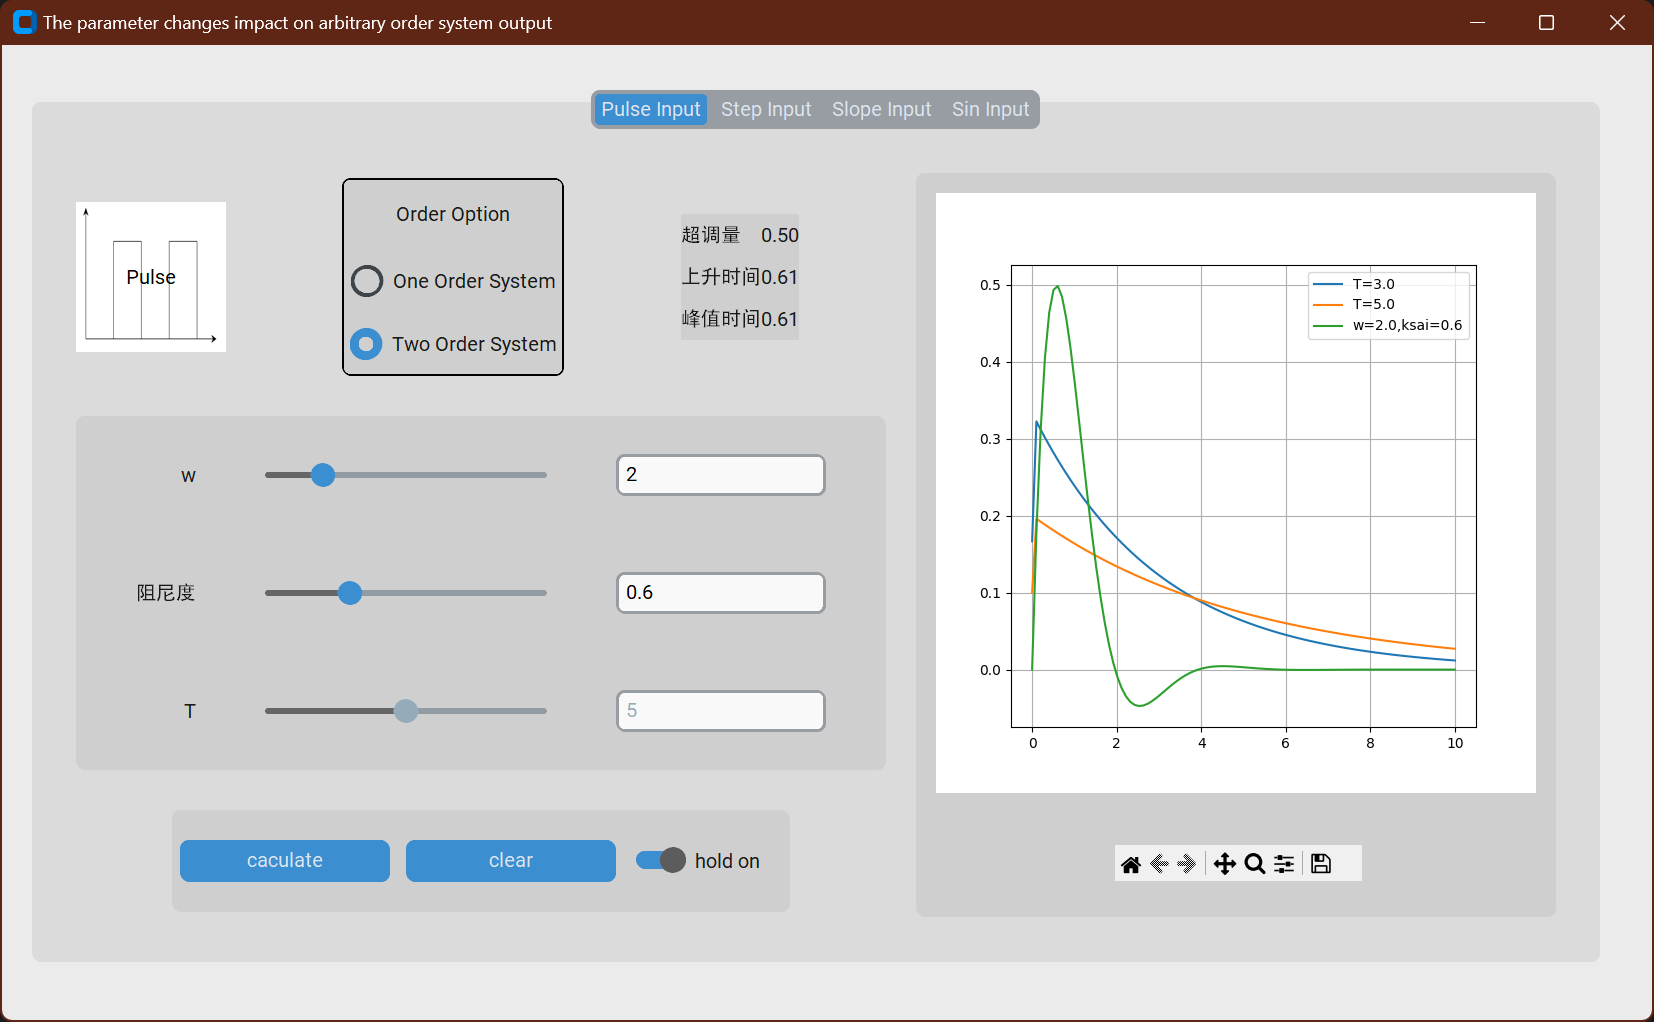
\includegraphics[width=0.7\textwidth]{img/static_draw.png}
    \caption{静态比较模式}\label{figure7}
\end{figure}

图\ref{figure7}展示了在静态曲线绘制模式下,T=3,T=5 两个一阶系统的响应曲线和 w=2.0,阻尼度(图中用“ksai”表示)=0.6 时,三种状态的响应曲线图比较

当 hold on 按钮状态显示关闭时,此时为曲线动态分析模式,该状态下“caculate”按钮显示为不可用,移动滑动条后会实时展示随着滑动条变化响应曲线的形状变化,同时也会在图例中更新对应参数,曲线动态分析模式见图\ref{figure8}所示。

\begin{figure}[htbp]
    \centering
    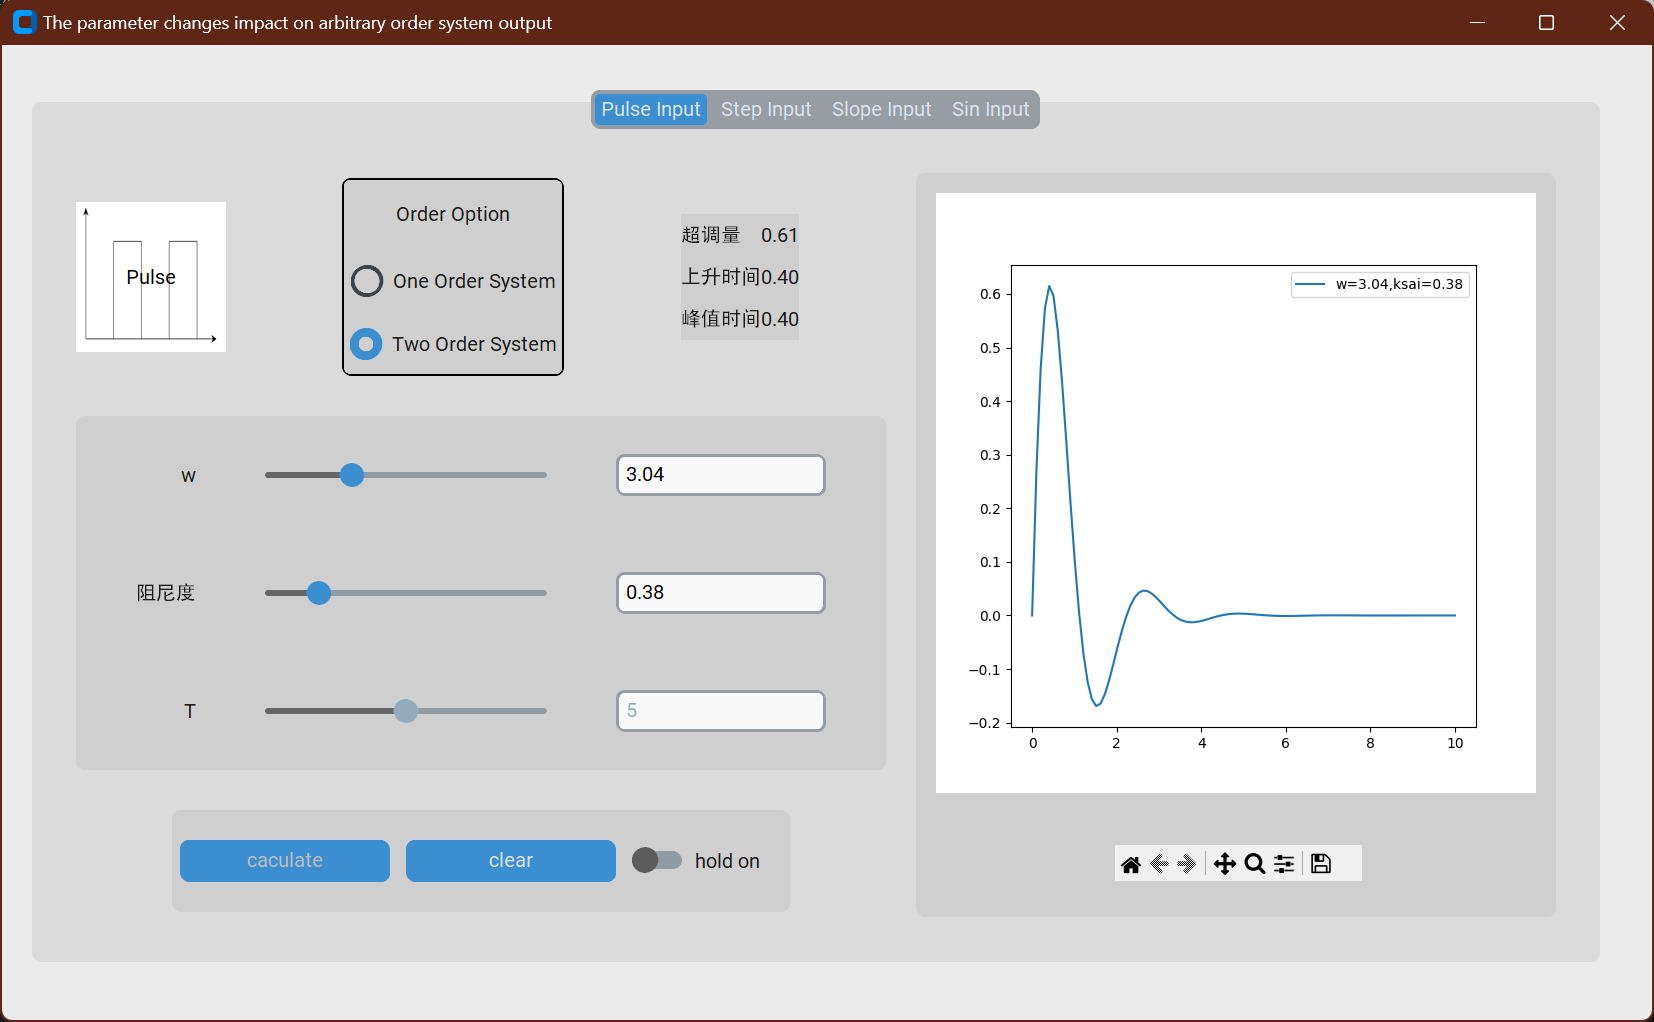
\includegraphics[width=0.7\textwidth]{img/dynamic.png}
    \caption{曲线动态分析模式}\label{figure8}
\end{figure}

一阶系统中,随着 T 的变化,状态响应曲线会实时改变;

二阶系统中,可以分别调整 w 和阻尼度,分别研究固有频率与阻尼度对响应曲线的影响。滑动条右侧的输入框内,既可以实时反映滑动条数值,也可以手动输入数据,使滑动条自动调整到用户输入的数值。

考虑到正弦信号输入的特殊性,本系统在正弦信号输入面板中,多加了信号频率参数,用来调节输入正弦信号的频率,如图\ref{figure9}所示。

\begin{figure}[htbp]
    \centering
    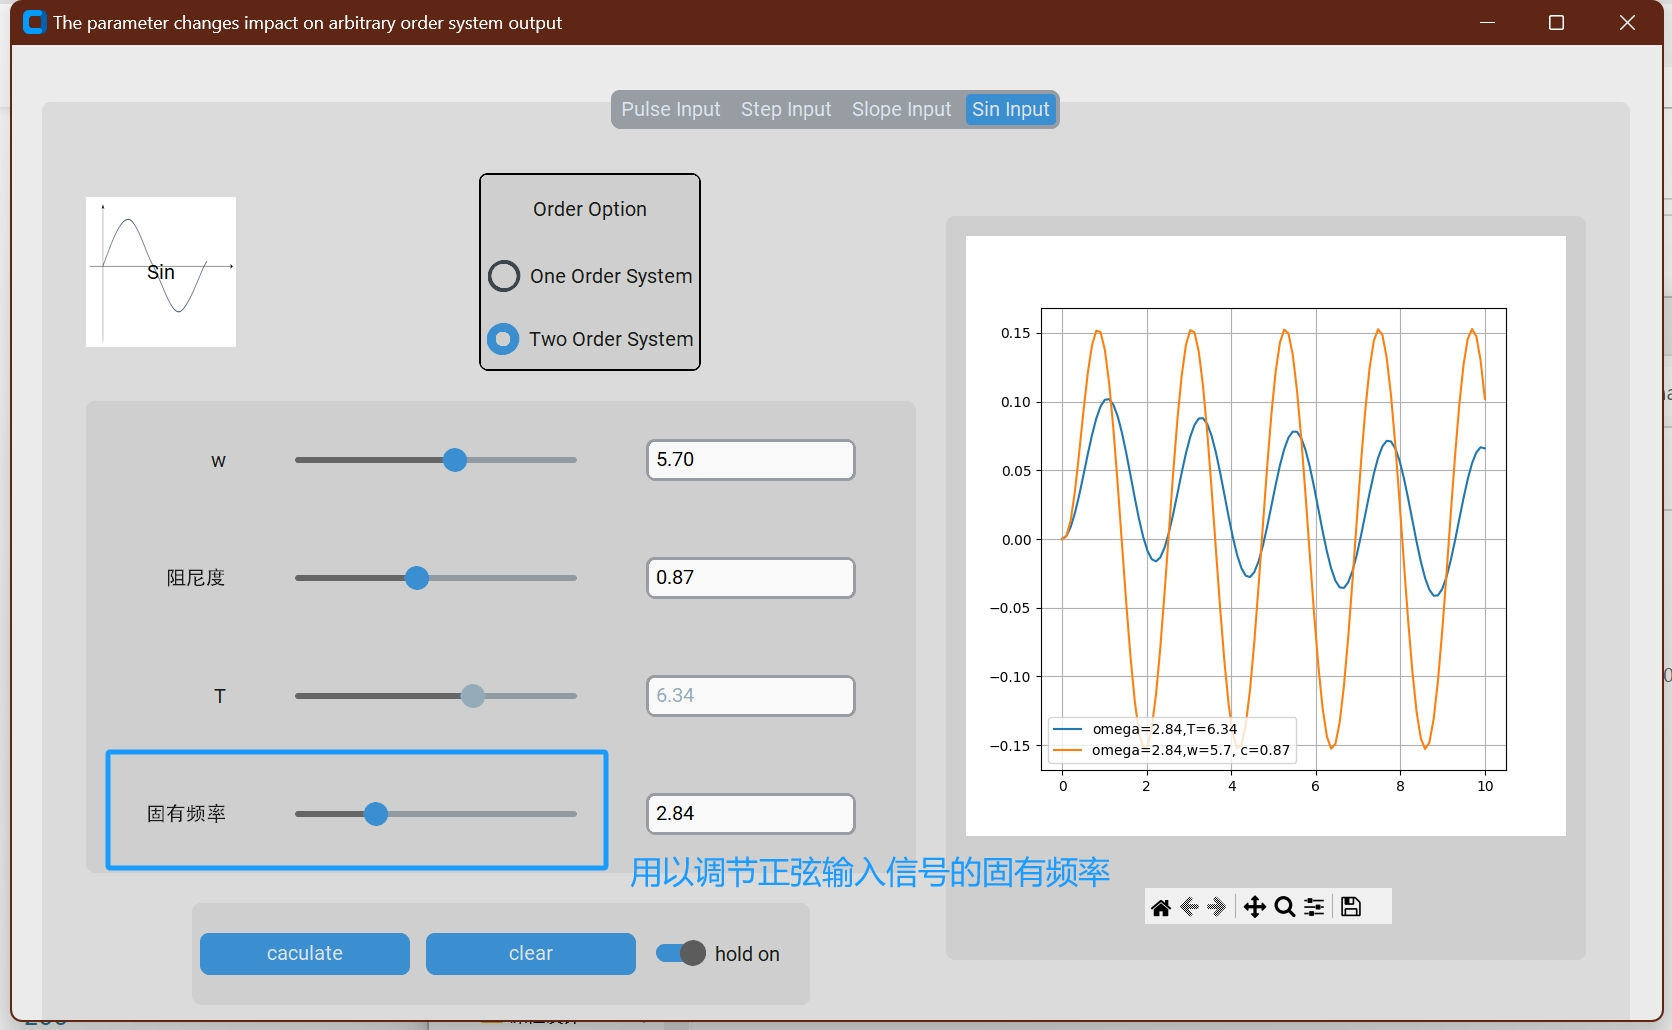
\includegraphics[width=0.7\textwidth]{img/sin_tab.png}
    \caption{正弦输入信号面板设计}\label{figure9}
\end{figure}

\section{系统前端代码实现}

\subsection{系统组件设计}

\subsubsection{输入信号模式指示器——Indicator 类}

本系统定义了\texttt{Indicator}类,用来指示每个面板的输入信号函数图像,方便用户理解。该输入信号模式指示器部署在每个面板的左上方,如图\ref{figure10}所示;本系统对“Pulse Input(脉冲输入) ” “Step Input(阶跃输入) ” “Slope Input(斜坡输入) ” “Sin Input(正弦输入)”四个信号的指示如图\ref{figure10}所示。

\begin{figure}[htbp]
    \centering
    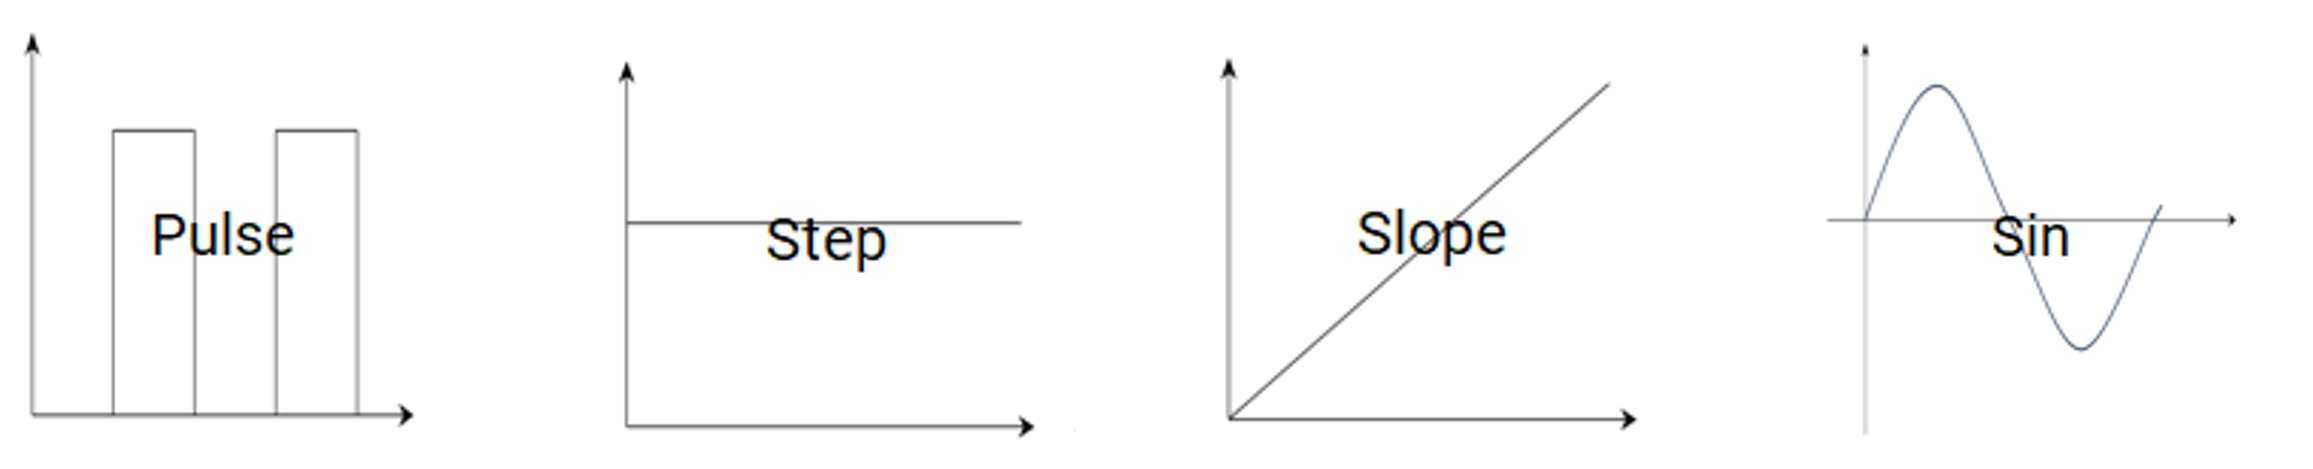
\includegraphics[width=0.7\textwidth]{img/input_indicator_img.png}
    \caption{输入信号指示图像}\label{figure10}
\end{figure}

Python 定义\texttt{Indicator}类代码为:

\begin{lstlisting}[title=Indicator 类代码]
import customtkinter
from PIL import Image
class Indicator(customtkinter.CTkFrame):
    def __init__(self, master: any, text: str, img_path: str, **kwargs):
        super().__init__(master, **kwargs)
        self.img = customtkinter.CTkImage(Image.open(img_path), size=(100, 100))
        self.label_img = customtkinter.CTkLabel(
            self,
            image=self.img,
            text=text.split(maxsplit=1)[0],
            width=50,
            height=50,
            text_color="#000000",
        )
        self.label_img.grid(row=0, column=0, padx=0, pady=0)
\end{lstlisting}

\subsubsection{指标显示容器—— metric 类}

本系统定义了\texttt{metric}类,用来作为系统准确性快速性指标布置容器,布置了“超调量”“上升时间”与“峰值时间”三个指标,在曲线动态分析模式下能够根据图像曲线实时显示曲线的相应指标,定义该类代码如下。
\begin{lstlisting}[title=metric 类代码]
import customtkinter
class metric(customtkinter.CTkFrame):
    def __init__(self, master: any, text: list[str], **kwargs):
        super().__init__(master, **kwargs)
        self.metric_text = [customtkinter.CTkLabel(self, text=j) for j in text]
        self.metric_val = [customtkinter.CTkLabel(self, text="") for j in text]
        for i, j in enumerate(self.metric_text):
            j.grid(row=i, column=0, sticky="w")
        for i, j in enumerate(self.metric_val):
            j.grid(row=i, column=1, sticky="w")
\end{lstlisting}

\subsubsection{按钮区——MyButton 类}

本系统定义了\texttt{MyButton}类,包含了 Caculate,Clear,Hold on 三个按钮,三个按钮的详细功能已在 3.2.2 中详细说明,此处不再赘述,定义\texttt{MyButton}代码如下所示。

\begin{lstlisting}[title=Mybutton 类代码]
    import customtkinter
    from core import one_order, Sin_one_order, two_order, Sin_two_order
    from draw import draw
    import numpy as np
    import matplotlib.pyplot as plt
    from metric_caculate import update
    
    global legend_on
    legend_on = []
    
    
    class MyButton(customtkinter.CTkFrame):
        def __init__(self, master: any, **kwargs):
            super().__init__(master, **kwargs)
            self.switch_var = customtkinter.IntVar(value=1)
            self.button = [
                customtkinter.CTkButton(self, text="caculate", command=self.draw_canvas),
                customtkinter.CTkButton(self, text="clear", command=self.clear),
                customtkinter.CTkSwitch(
                    self,
                    text="hold on",
                    variable=self.switch_var,
                    onvalue=1,
                    offvalue=0,
                    command=self.switch_disabled,
                ),
            ]
            for i, j in enumerate(self.button):
                j.grid(row=0, column=i, padx=5, pady=20)
    
        def caculate(self, v):
            f_plot = self.master.canvas.plot
            canvas = self.master.canvas.Canvas
            self.master.canvas.f.figure
            status = self.master.order_panel.selected.get()
            slider_block = self.master.slider_block
            metric = self.master.metric
    
            x, o_np = draw(canvas, f_plot, slider_block, status, v)
            update(metric, x, o_np)
    
        def sin_caculate(self, omega, T, w, c):
            f_plot = self.master.canvas.plot
            canvas = self.master.canvas.Canvas
            tab_name = self.master.master.master
            match self.master.order_panel.selected.get():
                case 0:
                    self.master.canvas.f.figure
                    o_np = Sin_one_order(omega, T)
                    x = np.linspace(0, 10, 100)
                    f_plot.plot(x, o_np(x))
                    legend_on.append("omega=%s,T=%s" % (str(omega), str(T)))
                    f_plot.legend(legend_on)
                case 1:
                    self.master.canvas.f.figure
                    o_np = Sin_two_order(omega, w, c)
                    x = np.linspace(0, 10, 100)
                    f_plot.plot(x, o_np(x))
                    legend_on.append("omega=%s,w=%s, c=%s" % (str(omega), str(w), str(c)))
                    f_plot.legend(legend_on)
            canvas.draw()
    
        def switch_disabled(self):
            f_plot = self.master.canvas.plot
            f_plot.cla()
            legend_on = []
            self.master.canvas.Canvas.draw()
            if self.button[2].get() == 0:
                self.button[0].configure(state="disabled")
            if self.button[2].get() == 1:
                self.button[0].configure(state="normal")
    
        def draw_canvas(self):
            tab_name = self.master.master.master
            w = self.master.slider_block.frame[0].x.get()
            c = self.master.slider_block.frame[1].x.get()
            T = self.master.slider_block.frame[2].x.get()
    
            for i, j in enumerate(["Pulse Input", "Step Input", "Slope Input"]):
                if tab_name.get() == j:  
                    self.caculate(v=i)
            if tab_name.get() == "Sin Input":
                omega = self.master.slider_block.frame[3].x.get()
                self.sin_caculate(omega=omega, T=T, w=w, c=c)
    
        def clear(self):
            f_plot = self.master.canvas.plot
            f_plot.cla()
            self.master.canvas.Canvas.draw()
\end{lstlisting}

\subsubsection{画布—— MyCanvas 类}

本系统定义了\texttt{MyCanvas}类,用来作为画布布置容器,配有一个曲线坐标图与导航栏,导航栏与图像链接,可以对曲线图像进行简单的变换操作,定义该类的代码如下:

\begin{lstlisting}[title=MyCanvas 类代码]
import customtkinter
from matplotlib.backends.backend_tkagg import FigureCanvasTkAgg, NavigationToolbar2Tk
from matplotlib.figure import Figure


class MyPlotNavigation(customtkinter.CTkFrame):
    def __init__(self, master: any, canvas, height=250, width=30, **kwargs):
        kwargs = {"fg_color": master._fg_color, **kwargs}
        super().__init__(master, height, width, **kwargs)
        self.toolbar = NavigationToolbar2Tk(canvas, self)
        self.toolbar.place(x=190, y=20, anchor=customtkinter.CENTER)


class MyCanvas(customtkinter.CTkFrame):
    def __init__(self, master: any, **kwargs):
        super().__init__(master, **kwargs)
        self.f = Figure(figsize=(6, 6), dpi=100)
        self.plot = self.f.add_subplot(111)
        self.plot.grid()

        self.Canvas = FigureCanvasTkAgg(self.f, self)
        self.Canvas.get_tk_widget().grid(row=0, column=0, padx=20, pady=20)
        self.toolbar = MyPlotNavigation(self, canvas=self.Canvas)
        self.toolbar.grid(row=1, column=0, padx=20, pady=20)
\end{lstlisting}

\subsubsection{系统阶数选择器——MyOrder 类}

本系统定义了\texttt{MyOrder}类,可以对系统的阶数进行选择,同时选择阶数后,将相应的参数滑动调节器启用,与该阶系统无关的参数滑动调节器停用,代码如下:

\begin{lstlisting}[title=MyOrder 类代码]
import logging

import customtkinter

from components.MySliderBlock import MySliderBlock


class MyOrder(customtkinter.CTkFrame):
    def __init__(
        self,
        master,
        title: str,
        button_name: list[str],
        ban: list[list[int]],
        sliderblock: MySliderBlock,
        **kwargs,
    ):
        assert button_name, "button_name can not be empty"
        kwargs = {
            "border_color": "black",
            "border_width": 1,
            **kwargs,
        }
        super().__init__(master, **kwargs)
        self.label = customtkinter.CTkLabel(self, text=title)
        self.label.grid(row=0, column=0, padx=20, pady=10)

        # define one order or two orders
        self.selected = customtkinter.IntVar(value=0)
        self.orders = [
            customtkinter.CTkRadioButton(
                self,
                command=self.callback,
                variable=self.selected,
                text=j,
                value=i,
            )
            for i, j in enumerate(button_name)
        ]
        for i, j in enumerate(self.orders):
            j.grid(row=i + 1, column=0, padx=5, pady=10)

        self.callback()
 
    def callback(self):
        logging.info("callback triggered, status:%d", self.selected.get())
        match self.selected.get():
            case 0:
                self.master.slider_block.set_enabled([False, False, True])
            case _:
                self.master.slider_block.set_enabled([True, True, False])
\end{lstlisting}

\subsubsection{系统参数滑动调节器——MySliderBlock 类}

本系统定义了\texttt{MySliderBlock}类,由三个部分组成:滑动条对应参数名称、滑动条、用户输入框,其中滑动条的数值与用户输入框内显示数值一致,可以通过输入框内数值读出参数值,也可在输入框内输入数值,将滑动条调整至需求位置,定义类代码如下:
\begin{lstlisting}[title=MySliderBlock 类代码]
import customtkinter
from core import Sin_one_order, Sin_two_order
from draw import draw_slider
import matplotlib.pyplot as plt
import numpy as np
from metric_caculate import update

global legend_on
legend_on = []


class MySlider(customtkinter.CTkFrame):
    def __init__(self, master: any, text: str, max, min, **kwargs):
        kwargs = { "fgcolor": master.fgcolor, **kwargs}
        super().__init__(master, **kwargs)
        # label
        self.label = customtkinter.CTkLabel(self, text=text)
        # slider
        self.x = customtkinter.DoubleVar(value=0.01)

        self.x_slider = customtkinter.CTkSlider(
            self, variable=self.x, from_=min, to=max, command=self.caculate
        )
        # entry
        self.x_entry = customtkinter.CTkEntry(self, textvariable=self.x)
        self.label.grid(row=0, column=0, padx=20, pady=20, sticky="w")
        self.x_slider.grid(row=0, column=1, padx=20, pady=20, columnspan=2, sticky="w")
        self.x_entry.grid(row=0, column=3, padx=20, pady=20, sticky="w")

    def set_enabled(self, state: bool):
        self.x_slider.configure(state="normal" if state else "disabled")
        self.x_slider.configure(button_color="#3B8ED0" if state else "#94acb9")
        self.x_entry.configure(state="normal" if state else "disabled")
        self.x_entry.configure(text_color="#000000" if state else "#94acb9")

    # button_color="#94acb9",
    # text_color="#b0b6b9",
    def draw_canvas(self, v, T, w, c):
        # T = self.master.slider_block.frame[2].x.get()

        global legend_on
        f_plot = self.master.master.canvas.plot
        Switch = self.master.master.button.button[2].get()
        canvas = self.master.master.canvas.Canvas
        # slider_block = self.master.master.slider_block
        status = self.master.master.order_panel.selected.get()
        metric = self.master.master.metric

        self.master.master.canvas.f.figure
        x, o_np = draw_slider(Switch, canvas, f_plot, status, v, T, w, c)
        if Switch == 0:
            update(metric, x, o_np)

    def sin_draw_canvas(self, T, omega, w, c):
        # T = self.master.slider_block.frame[2].x.get()

        global legend_on
        f_plot = self.master.master.canvas.plot
        self.master.master.canvas.f.figure
        if self.master.master.button.button[2].get() == 0:
            f_plot.clear()
        match self.master.master.order_panel.selected.get():
            case 0:
                o_np = Sin_one_order(omega, T)
                x = np.linspace(0, 10, 100)
                f_plot.plot(x, o_np(x))
                legend_on = ["omega=%s,T=%s" % (str(omega), str(format(T, ".2f")))]
                f_plot.legend(legend_on)
            case 1:
                o_np = Sin_two_order(omega, w, c)
                x = np.linspace(0, 10, 100)
                f_plot.plot(x, o_np(x))
                legend_on = ["omega=%s,w=%s,c=%s" % (str(omega), str(w), str(c))]
                f_plot.legend(legend_on)
        self.master.master.canvas.Canvas.draw()

    def caculate(self, value):
        self.x.set(format(value, ".2f"))
        # # f_plot = self.master.master.canvas.plot
        tab_name = self.master.master.master.master
        switch_val = self.master.master.button.button[2].get()
        status = self.master.master.order_panel.selected.get()
        for i, j in enumerate(["Pulse Input", "Step Input", "Slope Input"]):
            if tab_name.get() == j:
                if self.label._text == "w":
                    c = self.master.frame[1].x.get()
                    self.draw_canvas(v=i, w=value, c=c, T=0.01)
                if self.label._text == "zunidu":
                    w = self.master.frame[0].x.get()
                    self.draw_canvas(v=i, w=w, c=value, T=0.01)
                if self.label._text == "T":
                    T = self.master.frame[2].x.get()
                    self.draw_canvas(v=i, T=T, w=0.01, c=0.01)
                    # self.draw_canvas(v=i, T=value, w=0.01, c=0.01)

        if (
            tab_name.get() == "Sin Input"
            and switch_val == 0
            and self.label._text == "guyoupinlv"
            and status == 0
        ):
            T = self.master.frame[2].x.get()
            self.sin_draw_canvas(omega=value, T=T, w=0.01, c=0.01)

        if (
            tab_name.get() == "Sin Input"
            and switch_val == 0
            and self.label._text == "T"
            and status == 0
        ):
            omega = self.master.frame[3].x.get()
            self.sin_draw_canvas(omega=omega, T=value, w=0.01, c=0.01)
        if (
            tab_name.get() == "Sin Input"
            and switch_val == 0
            and self.label._text == "guyoupinlv"
            and status == 1
        ):
            w = self.master.frame[0].x.get()
            c = self.master.frame[1].x.get()
            self.sin_draw_canvas(omega=value, w=w, c=c, T=0.01)

        if (
            tab_name.get() == "Sin Input"
            and switch_val == 0
            and self.label._text == "w"
            and status == 1
        ):
            omega = self.master.frame[3].x.get()
            c = self.master.frame[1].x.get()
            self.sin_draw_canvas(omega=omega, w=value, c=c, T=0.01)

        if (
            tab_name.get() == "Sin Input"
            and switch_val == 0
            and self.label._text == "zunidu"
            and status == 1
        ):
            omega = self.master.frame[3].x.get()
            w = self.master.frame[0].x.get()
            self.sin_draw_canvas(omega=omega, w=w, c=value, T=0.01)
class MySliderBlock(customtkinter.CTkFrame):
    def __init__(
        self,
        master: any,
        text: list[str],
        max: list[float],
        min: list[float],
        *a,
        **kwargs
    ):
        super().__init__(master, *a, **kwargs)
        assert len(text) == len(max) and len(text) == len(
            min
        ), "arguments must have same length"
        self.frame = [MySlider(self, *i) for i in zip(text, max, min)]
        for i, j in enumerate(self.frame):
            j.grid(row=i + 1, column=0, padx=20, pady=5, sticky="e")

    def set_enabled(self, enabled: list[bool]):
        assert len(enabled) == len(self.frame), "arguments must have same length"
        for i, j in enumerate(self.frame):
            j.set_enabled(enabled[i])

	
\end{lstlisting}

\subsubsection{不同输入信号切换——TabView 与 tab_frame 类}

本系统包含“Pulse Input(脉冲输入) ” “Step Input(阶跃输入) ” “Slope Input(斜坡输入) ” “Sin Input(正弦输入)”四个面板,分别对应四种输入,利用 CustomTkinter 库的 CTkTabView 类,定义了\text{TabView}类,每个面板下,仅有一个\texttt{tab_frame}容器,用来放置每个面板下的控件,定义 \texttt{MyTab} 与 \text{tab_frame} 类代码如下:

\begin{lstlisting}[title=TabView 与 tab_frame 类代码]
import customtkinter
from .tab_frame import tab_frame
from .Sin_tab_frame import Sin_tab_frame
from .Indicator import Indicator
from .metric import metric
from .MyButton import MyButton
from .MyCanvas import MyCanvas
from .MyOrder import MyOrder
from .MySliderBlock import MySliderBlock

class MyTab(customtkinter.CTkTabview):
    def __init__(self, master: any, **kwargs):
        from components.tab_frame import tab_frame

        super().__init__(master, **kwargs)
        self.Pulse = self.add("Pulse Input")
        self.Step = self.add("Step Input")
        self.Slope = self.add("Slope Input")
        self.Sin = self.add("Sin Input")
        frame_args = {
            "slidertext": ["w", "zunidu", "T"],
            "max": [10, 2, 10],
            "min": [0.01, 0.01, 0.01],
        }
        self.frames = [
            tab_frame(
                self.Pulse,
                text="Pulse Signal Plot",
                img_path="img/pulse_signal.png",
                **frame_args
            ),
            tab_frame(
                self.Slope,
                text="Slope Signal Plot",
                img_path="img/slope_signal.png",
                **frame_args
            ),
            tab_frame(
                self.Step,
                text="Step Signal Plot",
                img_path="img/step_signal.png",
                **frame_args
            ),
        ]
        self.sin_frame = Sin_tab_frame(
            self.Sin,
            text="Sin Signal Plot",
            img_path="img/sin_signal.png",
            slidertext=["w", "zunidu", "T", "guyoupinlv"],
            max=[10, 2, 10, 10],
            min=[0.01, 0.01, 0.01, 0.01],
        )

        for i in self.frames:
            i.grid(row=0, column=0, padx=10, pady=10)
        self.sin_frame.grid(row=0, column=0, padx=10, pady=10)

    def get_frame_by_name(self, name: str):
        for i in self.frames:
            if i.name == name:
                return i

class tab_frame(customtkinter.CTkFrame):
    def __init__(
        self,
        master: any,
        text: str,
        slidertext: str,
        max: list[float],
        min: list[float],
        img_path: str,
        **kwargs
    ):
        assert len(max) == len(min), "arguments max and min must have same length"
        super().__init__(master, **kwargs)
        # Put indicator, orderoption, sliderblock, canvas, arguments
        self.indicator = Indicator(self, text=text, img_path=img_path)
        self.slider_block = MySliderBlock(self, text=slidertext, max=max, min=min)

        self.order_panel = MyOrder(
            self,
            title="Order Option",
            button_name=["One Order System", "Two Order System"],
            ban=[[0, 1], [2]],
            sliderblock=self.slider_block,
        )

        self.button = MyButton(self)
        self.canvas = MyCanvas(self)
        self.metric = metric(self, text=["chaotiao", "tr", "tp"])
        self.indicator.grid(row=0, column=0, padx=10, pady=10, sticky="w")
        self.order_panel.grid(row=0, column=1, padx=10, pady=10, sticky="w")
        self.slider_block.grid(row=1, column=0, padx=10, pady=10, columnspan=3)
        self.button.grid(row=2, column=0, padx=10, pady=10, columnspan=3)
        self.canvas.grid(row=0, column=4, padx=10, pady=10, rowspan=3)
        self.metric.grid(row=0, column=2, padx=10, pady=10, sticky="w")
\end{lstlisting}

同时,由于 Sin 信号的特殊性,需要考虑输入信号本身的频率特性,因此额外定义了\texttt{Sin_tab_frame}类用来部署 Sin 面板的控件,与\texttt{MyTab},\texttt{tab_frame}类类似,此处不再赘述。

\subsection{后端算法程序设计}

本系统中的前端空间回调函数均已包含在类的定义中,本系统分别对一阶二阶系统求反拉普拉斯的过程定义了函数,core.py 程序设计如下:

\begin{lstlisting}[title=core.py--inverse_laplace_transform]
import customtkinter
import matplotlib.pyplot as plt
from matplotlib.figure import Figure
import numpy as np
from sympy import *
from sympy.abc import t, s


def one_order(v, T):
    fun_input = 1 / s**v
    G = 1 / (T * s + 1)
    o = inverse_laplace_transform(fun_input * G, s, t)
    o_np = lambdify(t, o, "numpy")
    return o_np


def Sin_one_order(omega: float, T):
    sin_input = omega / (s**2 + omega**2)
    G = 1 / (T * s + 1)
    out = inverse_laplace_transform(sin_input * G, s, t)
    out_np = lambdify(t, out, "numpy")
    return out_np


def two_order(v, w, c):
    fun_input = 1 / s**v
    G = w / (s**2 + 2 * c * w * s + w**2)
    out = inverse_laplace_transform(fun_input * G, s, t)
    out_np = lambdify(t, out, "numpy")
    return out_np


def Sin_two_order(omega: float, w, c):
    sin_input = omega / (s**2 + omega**2)
    G = w / (s**2 + 2 * c * w * s + w**2)
    out = inverse_laplace_transform(sin_input * G, s, t)
    out_np = lambdify(t, out, "numpy")
    return out_np
\end{lstlisting}

而对准确性及快速性指标计算定义如下:

\begin{lstlisting}[title=metric_caculate.py]
import numpy as np
from components.metric import metric
from math import nan
from scipy.stats import randint
import sympy

def chaotiao(o_np):
    return np.max(np.abs(o_np))

def tp(x, o_np):
    return x[np.argmax(np.abs(o_np))]


def tr(x, o_np):
    return x[np.min(np.argmin(np.abs(o_np - 0.95)))]

def ts_step(T):
    return 4 * T


def update(metric: metric, x, o_np):
    metric.metric_val[0].configure(text=str(format(chaotiao(o_np), ".2f")))
    metric.metric_val[1].configure(text=str(format(tr(x, o_np), ".2f")))
    metric.metric_val[2].configure(text=str(format(tp(x, o_np), ".2f")))
\end{lstlisting}

\section{系统创新}
\begin{enumerate}
	\item 相较于MATLAB制作的传统GUI设计,本系统创新性地利用 Python 的 CustomTkinter 库设计了更为美观、易用的GUI程序,“易用”尤其体现在,MATLAB 的 Slider 控件,只能在鼠标拖动结束时运行回调函数,这样无法观察到在鼠标拖动过程中响应曲线的变化,相反,对 Python 的 CustomTkinter库而言,其提供的 Slider 滑动条在响应上更为迅捷,拖动过程中会不断运行回调函数,这样能够实时观察到在鼠标拖动过程中,也即参数连续变化过程中,响应曲线的实时变化,对动态性的研究更加充分。
	\item 本系统提供了两种模式,静态曲线绘制模式与曲线动态分析模式,为用户对比和比较响应曲线提供了便捷的方式,从静态和动态两个角度充分的对系统响应进行了研究,更加具有实际意义。
\end{enumerate}


\section{改进及不足}
\begin{enumerate}
	\item 本次课程设计中,在程序写作规范上还有待加强,有许多重复性的代码被反复复制粘贴,应该考虑加强函数或类的泛用性,来减少大量代码被重复使用的情况,精简程序;同时在对变量的命名上,缺乏规范,使变量名杂乱,可读性差,后续在代码训练过程中需要着重改进。
	\item 本次课程设计在sin正弦波输入信号面板中的后端算法亟待优化,在实际测试中发现,当hold on开关切到曲线动态分析模式时,响应曲线的图像变化非常卡顿,拖动滑动条会使程序陷入卡死停转的状态,原因一方面在于第一点所提到的程序结构不合理,另一方面在于后端算法需要改进优化,这需要在后续的学习中一步步找到解决方法。
	
	\item 本项目在系统准确性与快速性的计算上,还不够准确,需要精进对于Python sympy库的学习,通过曲线准确地分析超调量、上升时间、峰值时间、调整时间等物理参数。
\end{enumerate}

\section{心得体会}

\textbf{本次课程设计的Python代码全由本人一人独自编写},历时一周时间,中途有高中的同学的指点和帮助,当然也感谢网络上各类论坛的各类解答帮助我在碰到bug时能有效地解决他们。这次的课程设计也是我第一次接触如此复杂的项目,这个过程中学到了非常非常非常多的新知识,现将其列举如下:

\begin{enumerate}
	\item Python 语言

之前一直想要通过 Python 做一些程序和有用的东西出来,这一次课设是一个很好的契机,之所以会想到用 Python 的 CustomTkinter 库做这次课设,是因为偶然间发现了用 CustomTkinter 在 Github 上做的项目,看了 CustomTkinter 的帮助文档后发现其文档很详细,而且在 GUI 设计上比 MATLAB 要美观好看很多,就选择了他,在之后的使用中,越来越发现这个库相比于 MATLAB 的优越性。这次的学习也让我之后有了动力用Python去做一些自己喜欢的小程序,在写完这项课程设计之后,我们的机械设计基础的课程设计也开始了,我因为这次对 Python 的接触,代码能力显著提高,用 Python 写了一个程序来辅助我计算像齿轮直径、齿面弯曲疲劳等这些复杂的参数,有效地提高了课程设计效率。相较于一遍一遍地按计算器,我只需要在输入口,简单修改超参数的值(是的超参数!),如载荷系数,齿宽系数,传动比等这类人为定义的参数,在程序的辅助下能一分钟之内完成接下来一系列物理量的计算,大大帮助我提高了课程设计的效率。

	\item GIT版本控制系统

如前所述,在本次课程设计中有我高中同学的指导,他现在就读于华东理工大学的电子信息系,编程能力比我强得多,这就不可避免地会涉及远程协作,并且不断的修改需要版本控制系统来进行回档和 feature 的开发,借此机会我学习了GIT版本控制系统,也是在不断的摸索,查教程中学习的,这也帮助我在程序设计时,有效地回档、合并、协同工作,这些都大大地加快了我工作和学习效率,但是由于我也是第一次使用Git Graph,在commit的写作上还有所欠缺,很口语化,而并非是一个专业项目的注释,这也是日后需要我不断学习的地方,值得一提的是,下图是这个项目的Git Graph,最后一次提交是在12月1日晚00:30分,提交之后,我看着时间从November跳转到December才恍惚间意识到2023年的最后一个月已经来了,那是一个我忘不了的时刻,因为从那时开始,我在亲手创造些能为我所用的程序了,而不是被囿于单调的题目中。

\begin{figure}[htbp]
	\centering
	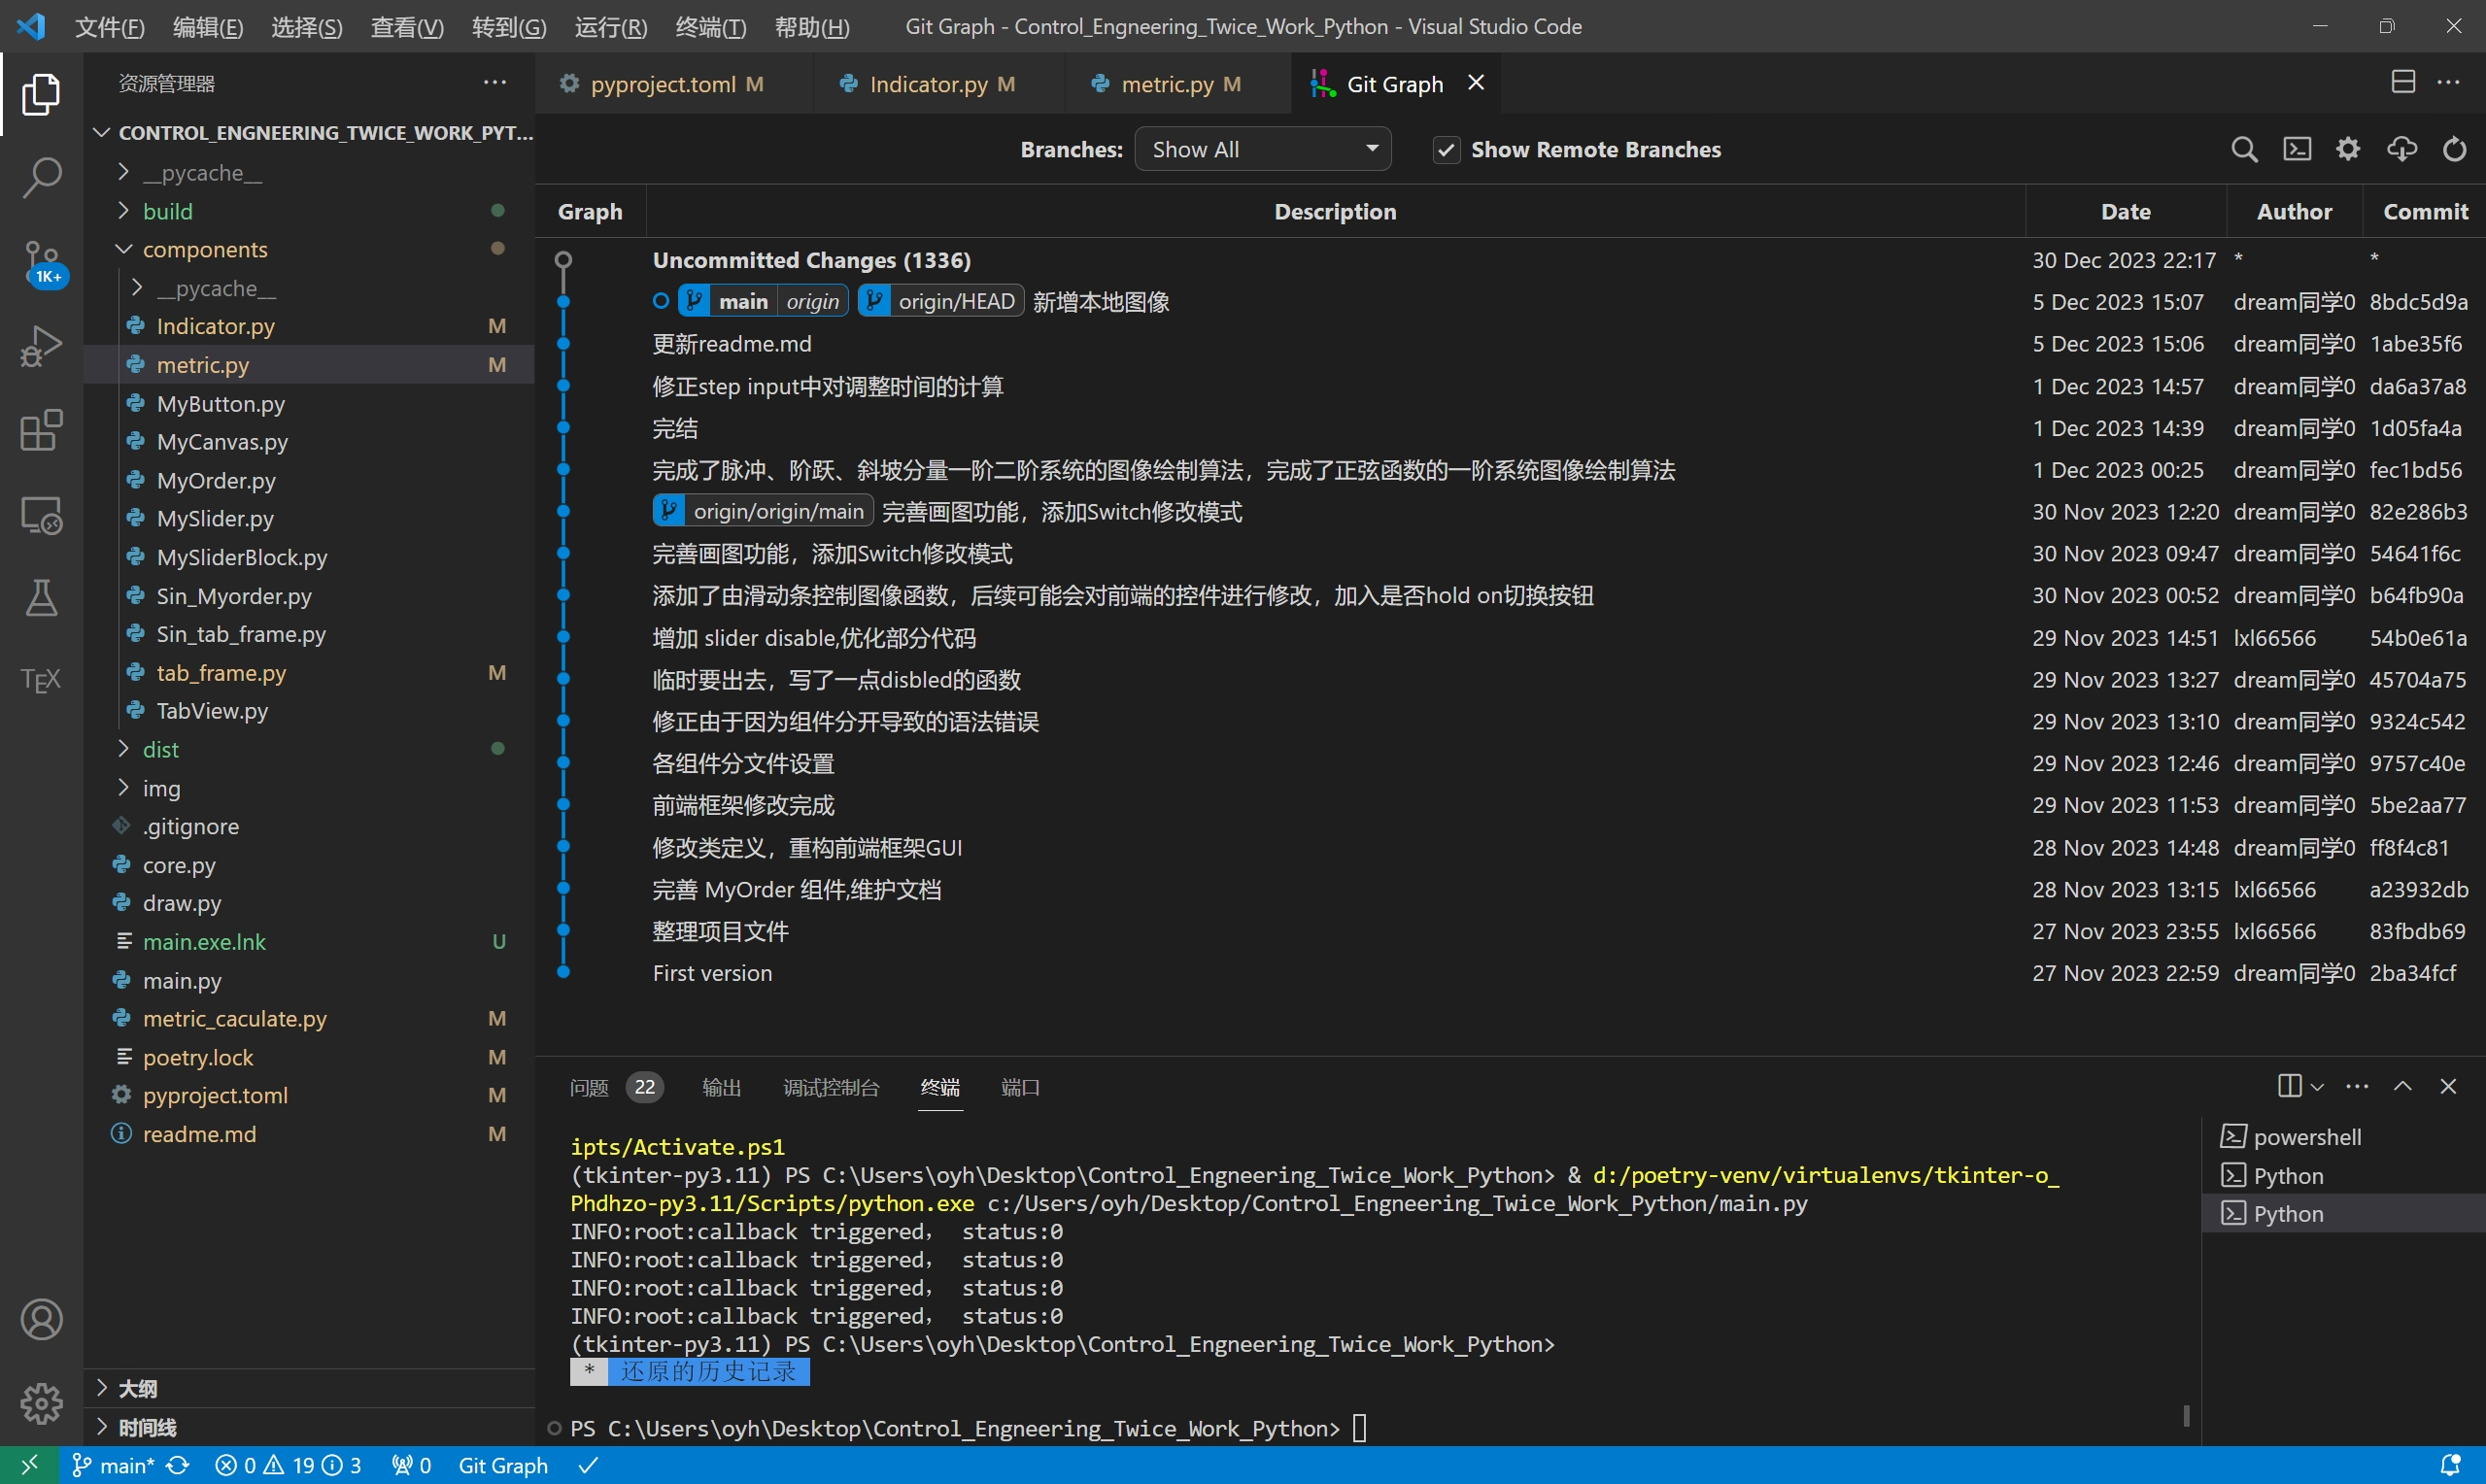
\includegraphics[width=0.7\textwidth]{img/GitGraph.png}
	\caption{Git版本控制树,该项目历经了十几个版本的迭代而成}
\end{figure}

	\item \LaTeX 写作

\textbf{本报告全篇均由我独自一人通过\LaTeX 撰写编译而得}。这是这个项目对我的最后一个挑战,和Python一样,之前也有很多次想要学一下\LaTeX 这门排版语言,但是也没有机会坚持学下去。这次的项目依旧给了我一个契机,让我开始学习\LaTeX 排版编程,期间在对图片和代码块的排版上出现了许多困难,我通过不断查找CSDN,Github 开源项目中的 issue,最终完成了这一篇报告的排版。这一过程很难,毕竟都是我从未接触过的技术与难题,但是不断克服困难的过程也让我感到惊喜和满足,不断挑战自己,努力向前,也会一直成为鼓励我向前走的不竭动力。

\end{enumerate}

感谢老师能阅读到此,这次的控制工程课程设计让我学会了很多从前想都不敢想的事,也感谢老师在这个学期里为我们授课,讲解控制工程知识,也希望控制工程这门课本身,能成为我的专业特长,成为今后突破难题的又一强有力的武器。

\end{document}
